This chapter will review what virtual reality is, how it is enabled through the use of virtual reality headsets and 
outline how virtual reality images are generated. After this, we will discuss some of the performance demands of virtual reality headsets 
and important considerations when designing and implementing virtual reality applications. 
We will also review the conditions \textit{simulator sickness} and \textit{virtual reality sickness}, which can be consequences of not adhering 
to the outlined considerations, and review ways to prevent this. More specifically we will discuss which factors that can be addressed in a virtual reality application's design and 
implementation phases, and which factors that are mostly due to individual differences and thus more outside the developers control. 
The lessons learned in this chapter will help guide the design and implementation consideration of the virtual reality design review application, which 
are discussed in chapter~\ref{chapter:design} and chapter~\ref{chapter:implementation}.


\section{The Basics of a Virtual Reality System}
\label{sec:vr_basics}
Virtual reality can be defined as a realistic and immersive simulation of a three-dimensional 360 degree environment, 
created using interactive software and hardware, and experienced or controlled by movement of the body~\citep{VRS2016}.

\begin{figure}%[h!] %[H]
	\includegraphics[width=\linewidth]{pictures/oculus_rift_dk1.jpg}
	\caption[The Oculus Rift Development Kit 1]{The Oculus Rift Development Kit 1, released by Oculus VR in 2012.}
	\label{fig:oculus}
\end{figure}

One of the most common ways to experience virtual reality is through virtual reality headsets, which are stereoscopic head-mounted displays (HMD) 
that provide separate images for each eye~\citep{POLYGON2016}. These head-mounted displays are fastened to the user's head using straps - similar to those employed by 
headlamps - and, once firmly in position, should cover the user's entire field of vision. 
Virtual reality headsets contain one display per eye, often referred to as a \textit{lenses}. These are positioned about 2-3 centimeters from their respective eye and have their own
associated camera in the virtual world, giving each eye its individual video feed. These cameras are offset by the same length as the distance between the user's eyes,
which enable depth vision and a true 3-dimensional experience~\citep{Abrash2012}. 

In addition to this, most virtual reality headsets also contain several head motion tracking sensors that are built into the headset. 
These detect any movement, and either moves or rotates the cameras in the virtual environment in unison with the user's head movement, thus enabling the user to turn
his or her head to "look around" in the virtual world~\citep{TW2016}. This usually includes a gyroscope, which is responsible for measuring the orientation of the
HMD, and sometimes an accelerometer to measure the proper acceleration of the HMD \citep{THEVERGE2016}. In addition, or instead of this, the first consumer versions of 
virtual reality headsets also usually utilize some other sensors or cameras outside the HMD. As an example the Oculus Rift CV1 utilizes constellation sensors~\citep{VRFOCUS2015}, 
which are usually positioned on a table, while the HTC Vive utilizes two Lighthouse Stations, which uses photosensors and 
structured light lasers to obtain the users position and rotation, and are usually placed in opposite corners of the room~\citep{GIZMODO2015}. 
Several virtual reality headset vendors also offer controllers that are either included or sold separately. These are usually wireless and 
utilize similar sensor technology as the head mounted devices.    

\begin{figure}%[h!] %[H]
	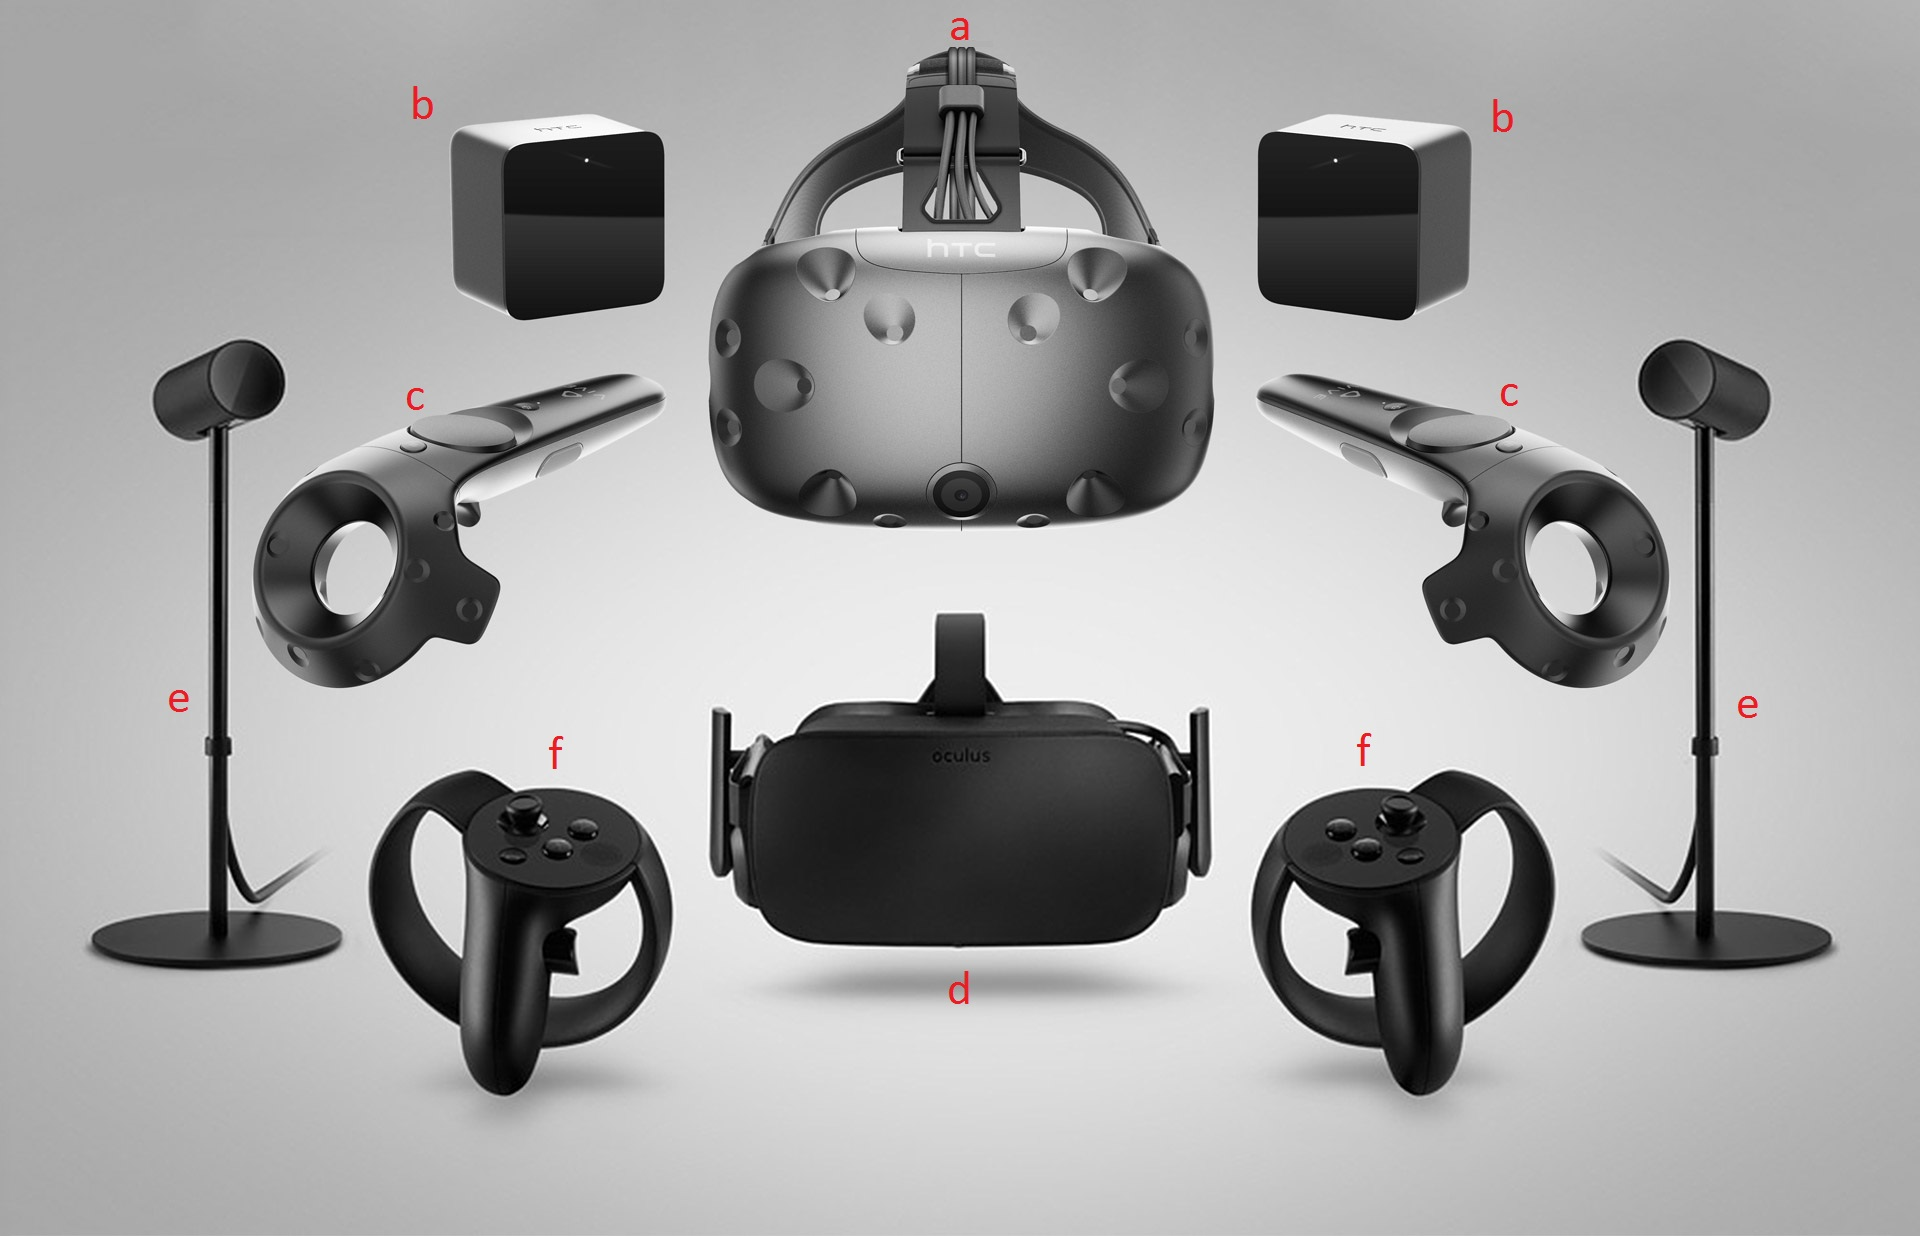
\includegraphics[width=\linewidth]{pictures/vive_and_rift_marked.jpg}
	\caption[The HTC Vive and Oculus Rift Hardware]{The HTC Vive and Oculus Rift Hardware. 
    a) The HTC Vive headset (HMD). b) The HTC Vive Lighthouse Stations. c) The HTC Vive Controllers. d) The Oculus Rift headset (HMD). e) The Oculus Rift Constellation Sensors. 
    f) The Oculus Rift Touch Controllers. Picture from \citet{ROADTOVR2016}}
	\label{fig:vive_and_rift_marked}
\end{figure} 

% Table med specs?

\subsection{Generating Virtual Reality Images}
There are a number of steps a virtual reality system has to perform from the moment a user performs an action to the moment that action is reflected visually on the displays.
The first step of this is head tracking. The HMD sensors and the tracking software have to determine the exact position and orientation of the HMD in the 
real world. Next, the application has to render the scene in stereo, i.e for both the cameras (as mention is section~\vref{sec:vr_basics}), 
as it would look from that point of view. As pixel density usually is low for HMDs with a wide field of view (more on that later), this step should usually 
also include anti-aliasing to avoid jagged edges and pixelation, and to ensure "smoother" images. When the application has rendered the frames/images (one per eye)
the frames need to be transfered to the HMD's displays by the graphics hardware. This is usually referred to as a scan-out and involves reading sequentially through the 
frame buffer, from top to bottom and moving right to left within each scan line, and streaming the pixel data for the scene over a link (e.g.~ a HDMI or Display Port cabel) 
to the displays~\citep{Abrash2012}. When the displays receive the pixel data they have to start emitting photons for each pixel, and, at some point, they 
have to stop emitting the photons to prepare for the next frames to be displayed. 


\section{Virtual Reality Performance Demands}
Virtual reality places some strict demands on performance and software design to avoid discomfort for the user. In many ways this is connected to how VR, 
as opposed to non-VR, applications "tricks" the user's brain into thinking the virtual experiences are actually real (giving it its "reality feel"). 
As a consequence of this, the user's brain tend to perceive VR-applications differently from non-VR application, e.g~by noticing anomalies more. 
One example of such an anomaly includes displacements of objects when the user's head rotates (i.e the objects are in the wrong position 
relative to the user's head)~\citep{Abrash2012}. 
Failing to meet the performance demands outlined below can quickly result in significant discomfort for the user and give symptoms like 
headache, nausea or disorientation. Many of these symptoms are also common in the closely related conditions \textit{simulator sickness} and \textit{virtual reality sickness},
which will be reviewed in section~\vref{sec:vr_sickness}.  
Before this we will discuss what generally makes virtual reality applications more demanding in terms of execution, design and implementation than non-VR applications.


\subsection{Latency Requirements}
Virtual reality headsets have a much stricter requirements for latency, i.e the time required for an input to have a visible effect, 
than with use of regular displays~\citep{ROADTOVR2013}. If this demand isn't met the system might often feel "sluggish" and the user will usually be more susceptible to
virtual reality sickness. %Latency plays a big role in the time required from a sensor registers a movement to that movement being reflected visually to the user.
If e.g.~too much time elapses between the time the user starts to turn his or her head, and the time 
the image is redrawn to account for the new head orientation, the visual image will feel disjoint for the user's action~\citep{Abrash2012}.

The virtual reality system should thus have as low latency as possible. 
\citet{Abrash2012}, an engineer behind the HTC Vive and currently a Chief Scientist at Oculus VR, wrote that "when it comes to VR and AR, latency is fundamental – 
if you don’t have low enough latency, it’s impossible to deliver good experiences, by which I mean virtual objects that your eyes and brain accept as real"
According to~\citet{Abrash2012} more than 20 milliseconds (ms) of latency is too much to be usable for virtual- and augmented reality, 
and a latency of 15 ms should be the absolute maximum.

One important component of latency is the \textit{refresh rates} of the displays, i.e 
how often the display hardware updates its buffers and thus "draws" a new image on the displays. Both the Oculus Rift CV1 and the HTC Vive
has a refresh rate of 90 Hz (i.e the display updates 90 times per second) for this reason, as opposed to the 60 Hz which is more common in commodity displays.
In addition to refresh rate, the \textit{frame rate}, i.e how often the graphics processing unit (GPU) renders new frames/images, is also important. To ensure 
that the displays don't "redraw" an identical frame on a buffer update the frame rate should thus ideally be the same or higher than the refresh 
rate (e.g 90 frames per second for the Oculus Rift CV1 or HTC Vive). Frame rate also determines the rendering latency, i.e the time is takes before 
an updated image, reflecting the user's latest actions, is produced. With 60 frames per second the rendering latency is on avaerage about 16.7 ms, while at 90 fps it is 
11 ms on average, and thus under the 15 ms maximum threshold (not accounting for other phases). %~\citep{Abrash2012}. 
Refresh rate and frame rate are thus highly codependent, where latency is only as low as the weaker of the two allow. 
The target computer should thus have a CPU and GPU strong enough to meet a frame rate equal or above to the HMD's refresh rate. 

\subsubsection{Asynchronous Reprojection}
To reduce the perceived latency, or to compensate for a frame rate that is too low, several virtual reality HMDs make use of \textit{asynchronous reprojection}
(equivalent to what Oculus VR refer to as "asynchronous time warp")~\citep{GD2016}. This is a technique in which the virtual reality system generates intermediate frames 
in situations where the software (e.g a game) can't maintained the required frame rate (which is typically 90 fps with 90 Hz). In simple terms asynchronous reprojection 
produces "in-between frames", which is a manipulated version of an older rendered frame. This is done my morphing the frame according to the most recent head tracking data just 
before the frame is presented on the displays~\citep{GD2016}. By doing this, software that runs at e.g 45 FPS (frames per seconds) natively can be transformed into 90 FPS by 
applying asynchronous reprojection to each rendered frame. Every other frame is thus actually a manipulated version of the former frame. It should be noted that frames produced by
asynchronous reprojection should only be regarded as "pseudo-frames" that compensation for lacking system performance in a rather performance-cost efficient manner, thereby
giving lower-end system (such as Sony's Playstation 4) access to VR. Also note that these pseudo-frames, produced by asynchronous reprojection, are still 
more susceptible to unfortunate side effects, such as \textit{positional judder}, than application rendered frames (the "real frames"). Positional judder is
one of the most obvious visual artifacts using this approach and can make objects near the user seem "blurry" or unfocused (see figure~\vref{fig:positional_judder})
~\citep{Antonov2015}. Asynchronous reprojection should thus only be regarded as a technique to compensate for a lacking frame rate, as its side effects are 
still considered better than the negative effects (such as latency) a low frame rate has for the virtual reality experience~\citep{OCULUS2016}. 

\begin{figure}%[h!] %[H]
	\label{fig:positional_judder}
	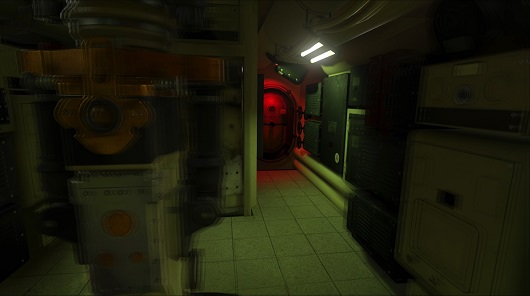
\includegraphics[width=\linewidth]{pictures/positional_judder.jpg}
	\caption[Positional judder can make objects near the user seem "blurry" or unfocused]
	{Positional judder can make objects near the user seem "blurry" or unfocused. In the image the objects near the user are more blurry than 
	than those that are farther away. This is because these object "move" more, relative to the user, from frame to frame as the user's head moves. 
	Picture from~\citet{Antonov2015}}
\end{figure} 


\subsection{Display Resolution and Pixel Density}
Virtual reality headsets also have strict demands in respect to display resolution and quality. As the eyes of the user is closer
to the displays than with a regular monitor, and the displays have to "wrap around" the user's whole field of view, flaws and shortcomings in the display technology 
become more apparent. 
One such example is the \textit{screen-door effect (SDE)}, which is when the lines separating the display pixel or subpixels are visible in the displayed image~\citep{TC2016}. 
To illustrate this issue \citet{TC2016} had the following remark about the Oculus Rift DK1 (released in 2013 with a resolution of 640×800 per eye):
"Its low resolution screen (combined with magnification lenses that helped wrap the image around your view) made even the most beautifully rendered 3D environment look dated. 
It was like you were sitting too close to an old TV, or staring at the display through a screen door (aptly, this shortcoming quickly came to be known as “the screen door effect”)"
With the release of commercial and more high-end virtual reality headset, the screen-door effect have become less apparent.
On the time of writing, two of the most sold virtual reality headsets, the Oculus Rift CV1 and the HTC Vive, both have a resolution of 1200 × 1080 per eye (a combined 
resolution of 2160 × 1200) with a pixel density of about 2450 ppi (pixel per inch), which is about ten times denser than the DK1's 215 ppi. 
With the improved pixel density, combined with the use of Fresnel lenses to create optical diffusion (i.e spreading out light to make it "softer"), 
the screen-door effect is severely minimized in the latest high-end virtual reality headsets~\citep{Davies2016}. 

\begin{figure}%[h!] %[H]
	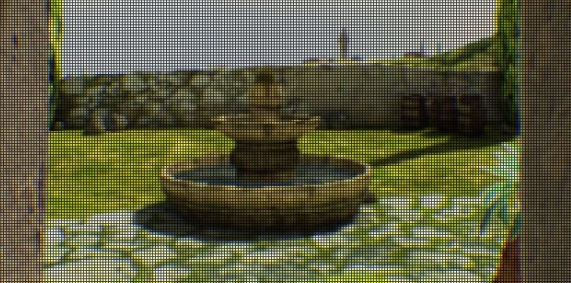
\includegraphics[width=\linewidth]{pictures/the_screen_door_effect.jpg}
	\caption[The screen-door effect]{An example of the screen-door effect.}
	\label{fig:the_screen_door_effect}
\end{figure} 

Just as having low latency, and thus a high amount of frames rendered per second, demands much from the computer, so does the high resolution.
As each lens has a resolution similar to a commodity computer display (1200 x 1080), the application must effectively render twice as many frames
as it would when only using such a display with the same frame- and refresh rate. With the 90 Hz refresh rate of the Rift and Vive, this effectively means
that 180 frames with a 1200 x 1080 resolution should ideally be produced per second.  

\subsection{Rendering Techniques}
In addition to the considerable hardware demands a virtual reality system places on a computer, it also impacts how virtual reality applications should be designed and implemented. 
This is specially apparent with rendering techniques, i.e the process of generating images from 2D or 3D models. 
As this is a demanding process with high fidelity graphics, as commonly found in modern computer games and other 3D applications, the rendering engine often employs several 
techniques and "tricks" to enhance it's performance, or at least make it seem so to the end user.
Several of these optimization techniques' value can be diminished in a virtual reality setting, thus not yielding the 
the same performance benefit as they would when applied to non-VR applications.

Because of the latest virtual reality headset's high resolution and wide field of view (usually about 110 degrees), 
more of the virtual environment is shown to the user in a frame than is usual in non-VR applications~\citep{Ohannessian2016}. 
This greatly affects several \textit{culling} techniques, such as \textit{frustum culling} and \textit{occlusion culling}), 
which are commonly used 3D rendering techniques for removing objects that don't contribute to the final image from the rendering pipeline~\citep{Johnson2013}.
Simply put, the rendering engine tries to only render what's actually visible to the user, while other objects are ignored by the rendering engine to diminish the workload. 
Frustum culling is concerned with only rendering objects that is within the field of view (the frustum pyramid) of user, while 
occlusion culling consists of filtering out the objects that are entirely hidden behind other opaque objects~\citep{PerezFernandez2015}. 
As, on average, more objects are visible to a user wearing a HMD than a user using a regular display more object have to be rendered, which implies a more work for the rendering
engine~\citep{Ohannessian2016}. 

Another commonly employed technique in game development is using flat 2D images for certain parts of the virtual environment instead of 3D objects~\citep{Ohannessian2016}.
Simple examples of this are e.g.~present in game "Super Mario 64", released for the Nintendo 64 in 1996, and one of the first commercially successful video games to utilize 3D.
In this game one can often spot objects, such as balls, trees and fences, that tries to appear as 3D objects, but in reality are 2D images that are rotated to always face the camera. 
Similar techniques, although usually more subtly applied, are still commonly used today, but not for virtual reality applications.
This is simply because the "2D deception" becomes much more obvious with the depth perception the stereo cameras enable~\citep{Ohannessian2016}. 


\section{Virtual Reality Sickness}
\label{sec:vr_sickness}
% Carsten: This is a very interesting survey of the state of knowledge in motion sickness. 
% Still, it should be motivated as well as concluded with some sentences that tell why this is an issue for your design, 
% and how the knowledge influences your design decisions. This discussion should be related to thesis goals that are already mentioned in section 1.3

Virtual reality sickness, a condition similar to \textit{simulator sickness}, 
can be a consequence of using virtual reality technology, and is considered a major barrier to 
using virtual reality. Like simulator sickness, virtual reality sickness causes symptoms that are similar to those of motion sickness, and can include symptoms like 
headache, stomach awareness, nausea, vomiting, pallor, sweating, fatigue, drowsiness and disorientation~\citep{Kolasinski1995}. 
To ensure an optimal virtual reality experience when using the design review application, the design and implementation should address these issues.
The following subsection will thus review what's known about virtual reality sickness and what can be done from a design and 
implementation standpoint.

Contrary to "regular" motion sickness, where the user visually perceived to be still while in actual motion, 
virtual reality sickness turns this around: The user visually perceive to be in motion which he or she is still. 
Virtual reality sickness can thus in many ways be considered as "a reverse motion sickness". Both these condition can thus be caused by
sensory conflict, i.e that there exist a discrepancy between the information given by the senses ("the human sensors").
The susceptibility for this condition vary widely among users. Some user might experience it shortly after putting on the headset, 
while others may never experience it~\citep{Stanney2003}.
The causes for virtual reality sickness can vary and while some are less under the VR application designer's control than others, 
they should still be understood by the VR designer~\citep{Stanney2003}. 
The following two subsections will review factors that contribute to virtual reality sickness, and make a distinction by
what are mostly determined by individual differences and whats mostly determined by the application design. 

\subsection{Individual Differences in Susceptibility}
Research has identified some individual differences that correlate with the individual's susceptibility for experiencing virtual reality sickness. 
One observation is that the susceptibility for virtual reality sickness correlates heavily with motion sickness susceptibility, and 
factors that influence motion sickness susceptibility also usually influence virtual reality sickness susceptibility~\citep{Stanney2003}.
Below are some theories of the major contributing factors that are based on individual differences, and which are difficult to account for during the design of a virtual reality application.

\subsubsection{Age}
Research suggest that users between the ages of 2 and 12 are the most susceptible to virtual reality sickness~\citep{Kolasinski1995}. The susceptibility then decreases
rapidly until an age of about 21, before it start decreasing more slowly until and age of 50, where the susceptibility increases again~\citep{Brooks2010}.

\subsubsection{Gender}
Women have proven more susceptible to virtual reality sickness than men~\citep{Kennedy1985}. The most common theories to explain this difference point out the genders' differences
in hormonal composition, field of view (some research suggest that women has a wider field of view than men) and differences in depth cue recognition~\citep{Biomed2012}. 
Women are most susceptible to virtual reality sickness during ovulation~\citep{Clemes2005}.

\subsubsection{Ethnicity}
Some ethnicities seem to be more susceptible to virtual reality sickness than others, suggesting a genetic component. 
Several studies indicate that asians tends to be more susceptible to visually-induced motion sickness,
with the Chinese being more susceptible that European-Americans and African-Americans on measures to motion sickness induced by a circular vection drum, and with
Tibetans and Northeast Indians having greater susceptibility than Caucasian races~\citep{Barrett2004}.

\subsubsection{Health}
Symptoms of virtual reality sickness are more prevalent in people who are fatigued, sleep deprived, are nauseated or have an upper respiratory illness, 
ear trouble or influenza~\citep{Kolasinski1995}.

\subsubsection{Postural Stability}
Users with a postural instability has been found to be more susceptible to visually-induced motion sickness, such as virtual reality sickness, and to experience
stronger symptoms of nausea and disorientation~\citep{Kolasinski1995}. 

\subsubsection{Experience with the Application}
More exposure to virtual environments can train the brain to be less sensitive to their effects~\citep{Stanney2003}. Users tend to become less likely to experience
virtual reality sickness as they become more familiar with the virtual reality application. This adaption may occur with only a few seconds of exposure to the application~\citep{Kennedy1985}.\\


In addition to this, people with a low threshold for detecting flicker and low mental rotation ability are more susceptible to virtual reality sickness~\cite{Kolasinski1995}.

\subsection{Virtual reality design factors}
This section identifies some of the most common contributers to virtual reality sickness that can be lessened or mitigated completely by the VR application design.

\subsubsection{Acceleration}
As mentioned earlier sensory conflict during a virtual reality session might occur. This is especially noticeable during acceleration that is conveyed visually, but 
not to the vestibular organs (inner ear organs that responds to acceleration). The speed of movement does not seem to contribute to virtual reality sickness in the same scale
as the vestibular organs do not respond to constant velocity. % Needs some references

\subsubsection{Camera Control}
Some theories indicates that the ability to anticipate and control the motion the user experiences plays a significant role in staving off motion- 
and virtual reality sickness~\citep{Rolnick1991}. Unexpected movement of the camera should thus be avoided in the virtual reality application. 
If the camera control is taken away from the user it is considered good practice to cue the impending camera movement to help the user to anticipate and prepare for 
the visual motion~\citep{Lin2004}.

\subsubsection{Field of View}
The term "field of view" (FOV) can refer both to \textit{display FOV} and \textit{camera FOV}, which are similar, 
but still distinct concepts that can both have an effect on the user's proneness to virtual reality sickness. 

Display FOV refers to the area of the visual field subtended by the display. As motion perception is more sensitive in the periphery view 
a wide display FOV can contribute to VR sickness by providing the visual system with more visual input, i.e more "area" in the periphery, than a smaller display FOV. 
This can lead to more sensory conflict as more of the visual view suggest that the user is moving, which he or she might be standing or sitting still.
Reducing display FOV can reduce the changes of VR sickness \citep{Draper2001}, but can also reduce the level of immersion and awareness, and require the user to turn his or her head more
than with a higher display FOV.

Camera FOV refers the area of the virtual environment that the graphics engine draws to the display.
If the camera FOV is setup wrong, movement of the user head can lead to unnatural movement in the virtual environment (e.g a 15° rotation of the head can lead to a 
25° rotation of the camera in the virtual environment). In addition to begin highly discomforting, this can lead to a temporary impairment in the vestibulo-ocular reflex, 
which is a reflex to stabilize images on the retinas during head movement~\citep{Stanney2002}.

\subsubsection{Focus Distance}
To avoid discomfort and fatigue it is important to place content the user will be focusing on for extended amounts of time in an optimal range.
As an example Oculus VR recommends such content to be placed a distance in the range of 0.75 to 3.5 Unity units/meters away from the camera \citep{OCULUS2016}. 

\subsubsection{Latency and Lag}
As mentioned earlier in this chapter, latency and lag can have a major impact VR sickness and the usability of the virtual reality application as a whole.
Although designers and developers have no control over many aspects of a system's performance, it's important to make sure the target virtual reality application
doesn't drop frames or lag on a minimum technical specifications system~\citep{OCULUS2016}. While some dropped frames or occasional jitter can be a minor annoyance
in conventional applications or video games, it can have a much more discomforting effect on the user of a virtual reality application. 

Some research indicates that a fixed, and thus predictable, latency creates about the same degree of VR sickness whether it's as short as 48 milliseconds or as long 
as 300 milliseconds, and that big and predictable latency or lag are more comfortable for VR users than smaller, but more unpredictable, latency or lag~\citep{Draper2001}. 

\subsubsection{Mouse and Keyboard Usage}
While a user is wearing a virtual reality headset, interaction with external input devices such as a keyboard, might be inconvenient or difficult. 
Put simply, this is because the user can't see his or her hands and thus can't get the visual hand positional feedback they could get without the virtual reality HMD. 
Because of this, many virtual reality applications makes use of a gamepad controller instead. %reference needed

%\subsubsection{Distortion Correction}

%\subsubsection{Flicker}

%\subsubsection{Independent Visual Backgrounds}

%\section{Ways to combat virtual reality Sickness}

\section{Considerations for the Design Review Application}
Throughout this chapter we have reviewed various aspects related to virtual reality. 

